\documentclass{article}

\usepackage[utf8]{inputenc}
\usepackage[T1]{fontenc}
\usepackage[norsk]{babel}

% Math stuff
\usepackage{amsmath}
\usepackage{amssymb}
\usepackage{tikz}
\usetikzlibrary{positioning}
\usetikzlibrary{arrows.meta}
% Allows writing theorems
\newtheorem{theorem}{Theorem}[section]

\title{Uoffisiell Eksamensforelesning i MA0301}
\author{Henrik Hørlück Berg}
\begin{document}

% Kommentar
\maketitle

\newpage
\section{Boolsk logikk}

I denne delen vil snakker en om (åpne) \textit{påstander} (propositions),
vanligvis representert i form av en eller flere av variablene $p, q, r, s$ og $t$.
Hver påstand kan da enten være sann, eller usann, og representerer enten ved ordene \textit{true}/\textit{false},
gjerne forkortet til $T/F$, eller $1/0$.\\
Men, vi vet ikke hvorvidt disse påstandene er sanne eller usanne, og er vanligvis heller ikke interesert i dette,
men ønsker heller å finne nye påstander, utledet av disse påstandene, som vi kan garantere er sanne, som kalles en \textit{tautologi},
eller garantere at de er usanne, som kalles en \textit{motsigelse} (contradiction).


\begin{displaymath}
    \begin{array}{|c c|c|c|c|}
        \hline
        p & q & p \to q & (p \to q) \to p & ((p \to q) \to p) \to p\\
        \hline
        1 & 1 & 1 & 1 & 1\\
        1 & 0 & 0 & 1 & 1\\
        0 & 1 & 1 & 0 & 1\\
        0 & 0 & 1 & 0 & 1\\
        \hline
    \end{array}
\end{displaymath}

\newpage
\section{Mengdelære}

Mengder er en samling med \textit{distinkte} elementer. De har stort sett de samme reglene
som boolsk logikk, og \href{https://www.wikipendium.no/MA0301_Elementary_Discrete_Mathematics#sets}{Wikipendium} beskriver dette godt.
Det er viktig å ha god kontroll på dette, grunnet mengdelæren er en byggesten for mange av de senere temaene.\\
Ting å kunne til eksamen:
\begin{itemize}
    \item Medlem i mengden: \(x\in A\), \(x\not\in B\)
    \item Delmengder: \(A \subset B, A\subseteq B, A\not\subset B, A \not\subseteq B\)
    \item Vise likhet: \(A=B \Leftrightarrow A\subseteq B \land B \subseteq A\)
    \item Kardinalitet (antall elementer i en mengde): \(|A|\)
    \item Den tomme mengde, \(\emptyset = \{\} \left(\neq \{\{\}\} = \{\emptyset\}\right)\)
    \item Potensmengde (Power set): \(\mathcal{P}(A) = \{a ~|~ a \subseteq A\}\)
    \item Kardinaliteten til potensmengden: \(|\mathcal{P}(A)| = 2^{|A|}\)\\
    En må også kunne begrunne dette.
    \item Union, snitt, symmetrisk differanse, gjerne ved venn-diagram: \(\cup, \cap, \triangle\)
    \item Regneregler (som er identisk med logikken)
\end{itemize}

% Skriv om setbuilder-notasjon
\noindent Viktig å få med seg at mengdene \(\{a, a, a, a\}\) og \(\{a\}\) er identiske. Samme for \(\{a, b, a\}\) og \(\{b, a\}\)

\subsection{Oppgaver}

\subsubsection{V2008 - Oppgave 3}
La $A$ og $B$ være to mengder. Skriv mengden
\[
(A\cup B)-(B-A)    
\]
på kortest mulig måte.

\paragraph*{Løsningsforslag}
Anbefaler å teste ut med venn-diagram først, for å få en intuisjon for forventet resultat.
\begin{align*}
    (A\cup B)-(B-A) &= (A\cup B)\cap \overline{(B\cap\overline{A})}\\
    &= (A\cup B)\cap (\overline{B}\cup A)\\
    &= A\cup (B\cap \overline{B})\\
    &= A \cup \emptyset\\
    &= A
\end{align*}

\subsubsection{TMA4140 - K2019 Oppgave 1}

Avgjør om følgende likhet av mendge holder for alle mendger $X$ med
delmendger $A,B,C,D \subseteq X$.
\[
\overline{A \cup ((\overline{A} \cup B)\cap (C\cup \overline{B})\cap (D\cup \overline{C}))} \cup (\overline{A} \cup D) = X   
\]

\paragraph*{Løsningsforslag} % TODO

\newpage
\section{Induksjon}

\subsection{Oppgaver}

\subsubsection{Exercise 12, Exercise set 6, spring 2019}
Show that if $u_n$ is defined recursively by the 
rules $u_1 = 1,u_2 = 5$ and for all $n>1,u_{n+1}= 5u_n -6u_{n-1}$, then $u_n = 3n-2n$ for all $n\in \mathbb{N}$
\paragraph*{Løsningsforslag}
Base step: Proving for $n=1$ and $n=2$:
\begin{align*}
    u_1 = 1\\
    3^1-2^1 = 1\\
    u_2 = 5\\
    3^2-2^2 = 5
\end{align*}
We have now proved the statement for $n=1$ and $n=2$, we can assume the truth of the statement for $S(1), S(2), \dots,S(k-1), S(k)$ and want to show that that indicates that $S(k+1)$ is true:
\begin{align*}
    u_{k+1} &= 5u_{k}-6u_{k-1}\\
    &= 5(3^k-2^k)-6(3^{k-1}-2^{k-1})\\
    &= 5(3^k)-5(2^k)-6(\dfrac{1}{3}3^k)+6(\dfrac{1}{2}2^k)\\
    &= 5(3^k)-5(2^k)-2(3^k)+3(2^k)\\
    &= 3(3^k)-2(2^k)\\
    &= 3^{k+1}-2^{k+1}
\end{align*}
And thus we have proven the truth of the statement for all $n \in \mathbb{N}$

\newpage
\section{Relasjoner og funksjoner}

Her er det Kartesiske produktet viktig. Både relasjoner og funksjoner er delmendger av det
kartesiske produktet. 

Viktige mendger: $\mathbb{N}, \mathbb{Z}, \mathbb{Q}, \mathbb{R}$, dette er mendger dere har vært borti i lang tid, bare at vi nå ser litt mer spesifikt på de.

For relasjoner må disse fire konseptene forstås, her er $A$ og $B$ mengder, og $R$ en relasjon mellom disse:
\paragraph*{Refleksivitet} $\forall_{a\in A} (a,a)\in R$
\paragraph*{Transitivitet} $(a,b) \in R\land (b,c)\in R \to (a,c) \in R$
\paragraph*{Symmetri} $(a,b)\in R \to (b,a) \in R$
\paragraph*{Anti-symmetri} $(a,b) \in R \land (b,a)\in R \to a=b$\\

\noindent Utdyp forskjell mellom symmetri og anti-symmetri med høyde-eksempel, og et hasse-diagram.

Refleksivitet, Transitivitet, og Symmetri gir en ekvivalensrelasjon, mens Refleksivitet, Transitivitet, og Anti-symmetri gir en partiell ordning.

Ekvivalensklasser, er en partisjonering av elementer i et set, hvor alle partisjonene er \enquote{like}, i forbindelse med ekvivalensrelasjonen.

\subsection{Funksjoner}

Funksjoner har dere jobbet mye med tidligere, gjerne i formen av $f(x) = x^2$ eller liknende. Her skal vi se på det litt mer generelt.
Formelt sett defineres en funksjon som $f:A\to B$ er en delmendge av $A \times B$ slik at det for enhver $a\in A$
finnes et unikt element $b\in B$, og vi skriver $b=f(a)$

Det er spesielt to egenskaper somer viktig å merke seg:

\paragraph*{Injektiv} Eller en-til-en, altså at det kun finnes maksimalt ett element i $A$ som peker til ethvert element i $B$. Vanlig å vise ved å sette $f(x)=f(y)$ og se om de kun finnes en løsning.
\paragraph*{Surjektiv} Eller \enquote{på}, som vil si at funksjonen dekker hele kodomenet, altså for alle $b\in B$, så finnes det en $a\in A$ slik at $f(a)=b$
\paragraph*{Bijektiv} En funksjon er bijektiv, dersom den er både injektiv og surjektiv.


\subsection{Oppgaver}

\subsubsection{V2016 – Oppgave 6}
Let $A$ be the set of all functions from $\mathbb{Z}_+$ to $\{1,2,3\}$

a) Oppgi egenskapene til en ekvivalensrelasjon

b) Define a relation $\mathcal{R}_1$ on $A$ by setting $f\mathcal{R}_1 g$ if and only if $f(5)=g(5)$. Vis at dette er en ekvivalensrelasjon.



\newpage
\section{Relasjoner og funksjoner}

Her er det Kartesiske produktet viktig. Både relasjoner og funksjoner er delmendger av det
kartesiske produktet. 

Viktige mendger: $\mathbb{N}, \mathbb{Z}, \mathbb{Q}, \mathbb{R}$, dette er mendger dere har vært borti i lang tid, bare at vi nå ser litt mer spesifikt på de.

For relasjoner må disse fire konseptene forstås, her er $A$ og $B$ mengder, og $R$ en relasjon mellom disse:
\paragraph*{Refleksivitet} $\forall_{a\in A} (a,a)\in R$
\paragraph*{Transitivitet} $(a,b) \in R\land (b,c)\in R \to (a,c) \in R$
\paragraph*{Symmetri} $(a,b)\in R \to (b,a) \in R$
\paragraph*{Anti-symmetri} $(a,b) \in R \land (b,a)\in R \to a=b$\\

\noindent Utdyp forskjell mellom symmetri og anti-symmetri med høyde-eksempel, og et hasse-diagram.

Refleksivitet, Transitivitet, og Symmetri gir en ekvivalensrelasjon, mens Refleksivitet, Transitivitet, og Anti-symmetri gir en partiell ordning.

Ekvivalensklasser, er en partisjonering av elementer i et set, hvor alle partisjonene er \enquote{like}, i forbindelse med ekvivalensrelasjonen.

\subsection{Funksjoner}

Funksjoner har dere jobbet mye med tidligere, gjerne i formen av $f(x) = x^2$ eller liknende. Her skal vi se på det litt mer generelt.
Formelt sett defineres en funksjon som $f:A\to B$ er en delmendge av $A \times B$ slik at det for enhver $a\in A$
finnes et unikt element $b\in B$, og vi skriver $b=f(a)$

Det er spesielt to egenskaper somer viktig å merke seg:

\paragraph*{Injektiv} Eller en-til-en, altså at det kun finnes maksimalt ett element i $A$ som peker til ethvert element i $B$. Vanlig å vise ved å sette $f(x)=f(y)$ og se om de kun finnes en løsning.
\paragraph*{Surjektiv} Eller \enquote{på}, som vil si at funksjonen dekker hele kodomenet, altså for alle $b\in B$, så finnes det en $a\in A$ slik at $f(a)=b$
\paragraph*{Bijektiv} En funksjon er bijektiv, dersom den er både injektiv og surjektiv.


\subsection{Oppgaver}

\subsubsection{V2016 – Oppgave 6}
Let $A$ be the set of all functions from $\mathbb{Z}_+$ to $\{1,2,3\}$

a) Oppgi egenskapene til en ekvivalensrelasjon

b) Define a relation $\mathcal{R}_1$ on $A$ by setting $f\mathcal{R}_1 g$ if and only if $f(5)=g(5)$. Vis at dette er en ekvivalensrelasjon.



\newpage
\section{Kombinatorikk}


\subsection{Oppgaver}
\subsubsection{TMA4140 - K2019, Oppgave 2a}
Hva er koeffisienten til leddet $x^4 y^6$ i polynomet $(2x-3y)^{10}$?

\paragraph*{Løsningsforslag}

Benytter Binomalteoremet
\[
(x+y)^n=\sum_{k=0}^{n}\binom{n}{k} x^k y^{n-k}
\]
Vi ønsker å se på ledd 4 i summen, der hvor $x$ har potens 4.
\begin{align}
    \binom{10}{4}(2x)^4(-3y)^6 &= \binom{10}{4}\cdot 2^4 \cdot x^4 \cdot (-3)^6 \cdot y^6\\
    &= \binom{10}{4}\cdot 2^4 \cdot (-3)^6 \cdot x^4 y^6\\
    &= \binom{10}{4} 2^4 3^6 \cdot x^4 y^6
\end{align}
Dermed har vi at koeffisienten blir $\binom{10}{4} 2^4 3^6 $

\subsubsection{TMA4140 - K2019, Oppgave 2b}
Hvor mange injektive funksjoner finnes det fra $\{1,2,3,4\}$ til $\{1,2,3,4,5,6,7,8\}$

\paragraph*{Løsningsforslag} 

Her må en huske definisjonen av en funksjon. Da har man for hvert element i definisjonsmengden/domenet 
ett valg i verdiområdet/kodomenet, som sammen utgjør bildet til funksjonen. Siden funksjonene skal være
injektive, blir det utvalg uten tilbakelegging, og siden det er fire elementer i domenet, og funksjonen
må ha et definert output for hvert element i domenet, må vi velge fire ganger. Dermed blir svaret:
\[
8\cdot 7 \cdot 6\cdot 5   
\]

\newpage
\section{Grafer}

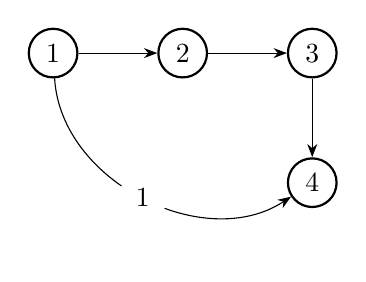
\begin{tikzpicture}
    \begin{scope}[every node/.style={circle,thick,draw}]
        \node(1){1};
        \node(2)[right=of 1] {2};
        \node(3)[right=of 2] {3};
        \node(4)[below=of 3] {4};
    \end{scope}
    %Lines
    \begin{scope}[>={Stealth[black]}, every node/.style={fill=white,circle}]
        \draw[->] (2.east) -- (3.west);
        \draw[->] (1.east) -- (2.west);
        \draw[->] (3.south) -- (4.north);
        \path [->] (1) edge[bend right=60] node {$1$} (4); 
    \end{scope}
    \end{tikzpicture}

\newpage
\section{Formelle språk og endelige tilstandsmaskiner}


\end{document}
